%------------------------------------------------------------------------------
% Master CV - Kamrul Hasan
% Author : Charles Rambo / Kamrul Hasan
% Template: photo-palatino-cv
% Compile with: pdflatex main_example.tex
%------------------------------------------------------------------------------

\documentclass[a4paper,11pt]{article}
\usepackage{latexsym}
\usepackage[empty]{fullpage}
\usepackage{titlesec}
\usepackage{marvosym}
\usepackage[usenames,dvipsnames]{color}
\usepackage{verbatim}
\usepackage{enumitem}
\usepackage[hidelinks]{hyperref}
\usepackage[english]{babel}
\usepackage{tabularx}
\usepackage{tikz}
\usepackage{graphicx}
\input{glyphtounicode}

% serif
\usepackage{palatino}

% Adjust margins
\addtolength{\oddsidemargin}{-1cm}
\addtolength{\evensidemargin}{-1cm}
\addtolength{\textwidth}{2cm}
\addtolength{\topmargin}{-1cm}
\addtolength{\textheight}{2cm}

\urlstyle{same}

\raggedbottom
\raggedright
\setlength{\tabcolsep}{0cm}

% Sections formatting
\titleformat{\section}{
  \vspace{-4pt}\scshape\raggedright\large
}{}{0em}{}[\color{black}\titlerule \vspace{-5pt}]

% Ensure that .pdf is machine readable/ATS parsable
\pdfgentounicode=1

%-----CUSTOM COMMANDS FOR FORMATTING SECTIONS----------------------------------
\newcommand{\CVItem}[1]{
  \item\small{
    {#1 \vspace{-2pt}}
  }
}

\newcommand{\CVSubheading}[4]{
  \vspace{-2pt}\item
    \begin{tabular*}{0.97\textwidth}[t]{l@{\extracolsep{\fill}}r}
      \textbf{#1} & #2 \\
      \small#3 & \small #4 \\
    \end{tabular*}\vspace{-7pt}
}

\newcommand{\CVSubSubheading}[2]{
    \item
    \begin{tabular*}{0.97\textwidth}{l@{\extracolsep{\fill}}r}
      \text{\small#1} & \text{\small #2} \\
    \end{tabular*}\vspace{-7pt}
}

\newcommand{\CVSubItem}[1]{\CVItem{#1}\vspace{-4pt}}

\renewcommand\labelitemii{$\vcenter{\hbox{\tiny$\bullet$}}$}

\newcommand{\CVSubHeadingListStart}{\begin{itemize}[leftmargin=0.5cm, label={}]}
\newcommand{\CVSubHeadingListEnd}{\end{itemize}}
\newcommand{\CVItemListStart}{\begin{itemize}}
\newcommand{\CVItemListEnd}{\end{itemize}\vspace{-5pt}}

%------------------------------------------------------------------------------
% CV STARTS HERE
%------------------------------------------------------------------------------
\begin{document}

%-----HEADING WITH PHOTO-------------------------------------------------------
\begin{minipage}[c]{0.05\textwidth}
\-\
\end{minipage}
\begin{minipage}[c]{0.2\textwidth}
\begin{tikzpicture}
    \clip (0,0) circle (1.75cm);
    \node at (0,-.7) {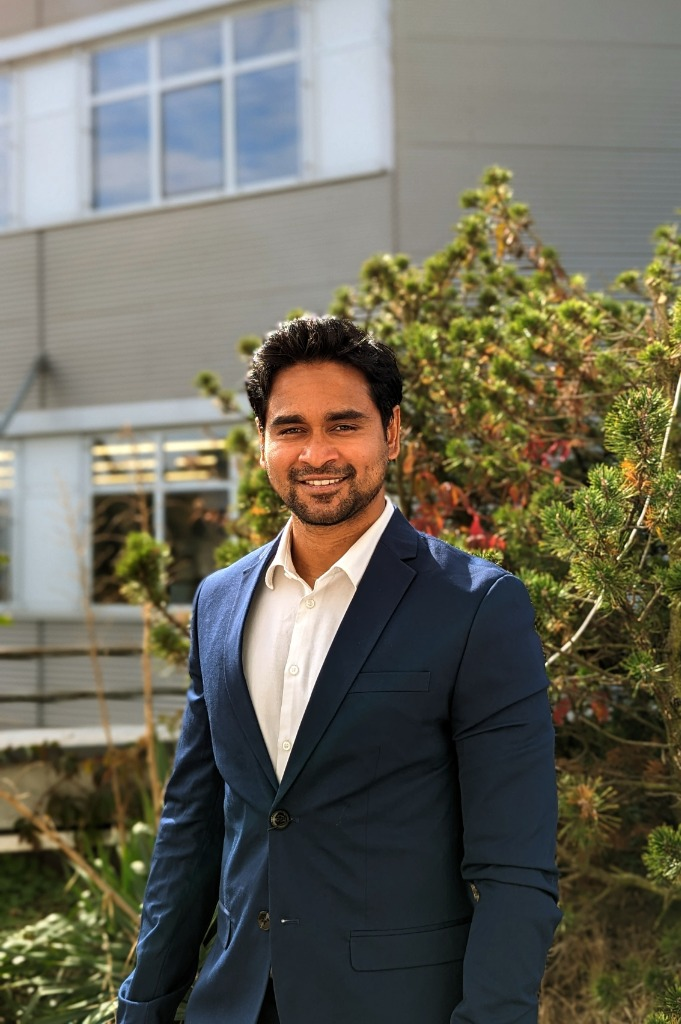
\includegraphics[width = 7cm]{formalP.jpg}}; 
\end{tikzpicture}
\hfill\vline\hfill
\end{minipage}
\begin{minipage}[c]{0.65\textwidth}
    \textbf{\Huge \scshape{Kamrul Hasan}} \\ \vspace{2pt} 
    \small{+49 1632304846} \\
    \href{mailto:haasankamrul14@gmail.com}{\underline{haasankamrul14@gmail.com}}\\
    \href{https://www.linkedin.com/in/kamrul-hasan}{\underline{linkedin.com/in/kamrul-hasan}} \\
    \href{https://github.com/kamrulroky}{\underline{https://github.com/kamrulroky}}
\end{minipage}

%-----EDUCATION----------------------------------------------------------------
\section{Education}
  \CVSubHeadingListStart
    \CVSubheading
      {{Master of Science $|$ \emph{\small{International Software Systems Science}}}}{2020 -- 2024}
      {Otto-Friedrich-Universität Bamberg}{Bamberg, Germany}
      \CVItemListStart
        \CVItem{Grade: 2.5 (GUT / GOOD). Focus: Distributed Systems, Mobile Systems, Complex Event Processing, Machine Learning.}
        \CVItem{Thesis: ``Enhancing RSSI-based Positioning Accuracy using Advanced Filtering Techniques'' (Grade: 3.2).}
      \CVItemListEnd
    \CVSubheading
      {{Bachelor of Science $|$ \emph{\small{Computer Science and Engineering}}}}{2012 -- 2017}
      {Stamford University Bangladesh}{Dhaka, Bangladesh}
      \CVItemListStart
        \CVItem{Thesis: ``Applications of Internet of Things Towards Smart Home Automation.''}
      \CVItemListEnd
  \CVSubHeadingListEnd

%-----WORK EXPERIENCE----------------------------------------------------------
\section{Work Experience}
  \CVSubHeadingListStart
    \CVSubheading
      {Research Engineer (Wissenschaftlicher Mitarbeiter)}{May 2024 -- April 2026}
      {Institut für Systems Engineering für zukünftige Mobilität (DLR)}{Oldenburg, Germany}
      \CVItemListStart
        \CVItem{Developed research software for runtime validation of Automated Driving Systems (ADS), integrating multi-sensor and infrastructure hazard data into evaluation pipelines.}
        \CVItem{Designed scenario-based verification pipelines in CARLA simulation and implemented validation metrics for monitoring ADS safety.}
        \CVItem{Implemented and evaluated middleware for workload and container orchestration on embedded platforms (Eclipse Ankaios, ROS2, Embedded Linux).}
        \CVItem{Collaborated with consortium stakeholders to translate scientific objectives into deployable prototypes; authored IEEE IV 2026 paper.}
      \CVItemListEnd

    \CVSubheading
      {Embedded and Backend Developer (Werkstudent)}{December 2020 -- April 2024}
      {Favendo GmbH}{Bamberg, Germany}
      \CVItemListStart
        \CVItem{Developed indoor/outdoor positioning algorithms using advanced Kalman and particle filtering techniques for commercial RTLS.}
        \CVItem{Designed and validated embedded firmware for positioning sensors; conducted unit, integration, and system testing for multi-sensor hardware.}
        \CVItem{Analyzed and improved positioning accuracy through systematic measurement calibration and reliability characterization.}
      \CVItemListEnd

    \CVSubheading
      {Software Engineer}{November 2018 -- September 2020}
      {LEADS Corporation Ltd.}{Dhaka, Bangladesh}
      \CVItemListStart
        \CVItem{Researched, developed, and deployed software solutions for IoT and AI-driven applications.}
        \CVItem{Enhanced software development lifecycle practices by adopting Agile and Scrum methodologies.}
      \CVItemListEnd

    \CVSubheading
      {Embedded Software Engineer}{May 2017 -- October 2018}
      {JolPi Electronics Ltd.}{Dhaka, Bangladesh}
      \CVItemListStart
        \CVItem{Developed and debugged embedded software utilizing FreeRTOS and bare-metal C programming for ARM microcontrollers.}
        \CVItem{Applied Test-Driven Development (TDD) to firmware design and board bring-up for consumer electronic devices.}
      \CVItemListEnd
  \CVSubHeadingListEnd

%-----SKILLS-------------------------------------------------------------------
\section{Technical Skills}
 \begin{itemize}[leftmargin=0.5cm, label={}]
    \small{\item{
     \textbf{Programming Languages}{: C/C++, Python, Bash, MATLAB, UML} \\
     \textbf{Research \& System Engineering}{: System Design \& Modeling, Verification \& Validation (V\&V), Technical Standards} \\
     \textbf{Platforms and Frameworks}{: ROS2, CARLA, FreeRTOS, OpenCV, Embedded Linux, QEMU, TensorFlow, Eclipse Ankaios} \\
     \textbf{Development Tools}{: GNU Toolchain, CMake, Docker, Git, Ansible, OpenOCD, JTAG, LaTeX, Confluence, Jira, Claude Code} \\
     \textbf{Development Hardware}{: STM32, Raspberry Pi, Jetson Orin, RISC-V, ARM Cortex, ESP32/ESP8266, Simulation PC} \\
     \textbf{Technologies}{: Interfaces \& Protocols, Sensor Fusion, Computer Vision, Wireless Communication, Analog \& Digital Electronics, PCB (Altium)} \\
     \textbf{Industry Knowledge}{: Distributed Systems, APIs, Agentic AI, SCRUM, Simulation, Hardware-in-the-Loop (HIL)} \\
    }}
 \end{itemize}

%-----PROJECTS AND RESEARCH----------------------------------------------------
\section{Publication and Scientific Writing}
  \CVSubHeadingListStart
    \CVSubheading
      {\href{https://ieeexplore.ieee.org/document/11624101}{Leveraging External Hazard Data to Safeguard Automated Driving System}}{}
      {IEEE Intelligent Vehicles Symposium (IV 2026)}{}
    \CVSubheading
      {\href{https://www.researchgate.net/publication/400899464_Enhanching_RSSI-based_Positioning_Accuracy_using_Advanced_Filtering_Techniques}{Enhancing RSSI-based Positioning Accuracy using Advanced Filtering Techniques}}{}
      {Master Thesis $|$ Otto-Friedrich-Universität Bamberg}{}
    \CVSubheading
      {\href{https://www.researchgate.net/publication/400899541_Applications_of_Internet_of_Things_Towards_Smart_Home_Automation}{Applications of Internet of Things Towards Smart Home Automation}}{}
      {Bachelor Thesis $|$ Stamford University Bangladesh}{}
    \CVSubheading
      {On Device Smart Assistant Using Mozilla DeepSpeech}{}
      {Case Study}{}
  \CVSubHeadingListEnd

%-----CERTIFICATION AND AWARDS-------------------------------------------------
\section{Certification and Awards}
  \CVSubHeadingListStart
    \CVSubheading
      {Silver Medal Winner -- International Blockchain Olympiad (IBCOL 2020)}{Hong Kong}
      {Awarded for innovative blockchain-IoT architecture}{}
    \CVSubheading
      {Certified IoT Engineer}{Dhaka, Bangladesh}
      {Bangladesh Computer Council (BCC), LICT Project}{}
    \CVSubheading
      {AI Programming with Python Nanodegree}{Online}
      {Udacity}{}
  \CVSubHeadingListEnd

%-----COMPETENCIES & ACTIVITIES------------------------------------------------
\section{Competencies \& Activities}
 \begin{itemize}[leftmargin=0.5cm, label={}]
    \small{\item{
     \textbf{Languages}{: English (CEFR C1 -- Full Professional), Deutsch (CEFR A2), Bengali (Native), Hindi (Conversational)} \\
     \textbf{Soft Skills}{: Analytical Thinking, Self Management, Cross-Functional Teamwork, Technical Communication} \\
     \textbf{Others}{: Driving License, PC Building, Hobbyist Hardware Maker} \\
    }}
 \end{itemize}

\end{document}
